% Document Type
\documentclass[a4paper,11pt]{article}

% Packages
\usepackage{latexsym}
\usepackage[empty]{fullpage}
\usepackage{titlesec}
\usepackage{marvosym}
\usepackage[usenames,dvipsnames]{color}
\usepackage{verbatim}
\usepackage{enumitem}
\usepackage{fancyhdr}
\usepackage[english]{babel}
\usepackage{tabularx}
\usepackage{graphicx}
\usepackage{color}
\usepackage[table]{xcolor}
% \usepackage{tgbonum}
\usepackage[sfdefault]{ClearSans} %% option 'sfdefault' activates Clear Sans as the default text font
\usepackage[T1]{fontenc}
\usepackage[margin=1.4in]{geometry}
\usepackage{setspace}
\usepackage{multirow}
\usepackage[hidelinks]{hyperref}
\input{glyphtounicode}

% Cover Information
\title{Ling Li Ya CV}
\author{Ling Li Ya}
\date{\today}


\pagestyle{fancy}
\fancyhf{} % clear all header and footer fields
\fancyfoot{}
\renewcommand{\headrulewidth}{0pt}
\renewcommand{\footrulewidth}{0pt}


% My Colours
\definecolor{MyBlue}{rgb}{0.17, 0.27, 0.59}
\definecolor{MyBGColor}{rgb}{0.90, 0.94, 0.98}
\definecolor{MyHighlight}{rgb}{1.00, 0.89, 0.00}


% URL
\hypersetup{breaklinks=false,%
% pagecolor=white,%
colorlinks=true,%
linkcolor=MyBlue,%
anchorcolor=MyBlue,%
urlcolor=MyBlue}
\urlstyle{same}


% Adjust margins
\addtolength{\oddsidemargin}{-0.5in}
\addtolength{\evensidemargin}{-0.5in}
\addtolength{\textwidth}{1in}
\addtolength{\topmargin}{-0.7in}
\addtolength{\textheight}{1.0in}

\raggedbottom
\raggedright
\setlength{\tabcolsep}{0in}


% Sections formatting
\titleformat{\section}{
  \vspace{5pt}\raggedright\large\bfseries
}{}{0em}{}[\color{black}\titlerule \vspace{-5pt}]


% Ensure that generate pdf is machine readable/ATS parsable
\pdfgentounicode=1


%-------------------------
% Custom commands
\newcommand{\resumeItem}[2]{
  \item\small{
    {#1}{#2 \vspace{-2pt}}
  }
}


% Just in case someone needs a heading that does not need to be in a list
\newcommand{\resumeHeading}[4]{
    \begin{tabular*}{0.99\textwidth}[t]{l@{\extracolsep{\fill}}r}
      \textbf{#1} & {#2} \\
      \textit{\small#3} & \textit{\footnotesize #4} \\
    \end{tabular*}\vspace{-5pt}
}


\newcommand{\resumeSubheading}[4]{
  \vspace{-1pt}\item
    \begin{tabular*}{0.97\textwidth}[t]{l@{\extracolsep{\fill}}r}
      \textbf{\color{MyBlue} #1} & {\footnotesize#2} \\
      \textit{\footnotesize #3} & \textit{\footnotesize #4} \\
    \end{tabular*}\vspace{-5pt}
}


\newcommand{\resumeSubSubheading}[2]{
    \begin{tabular*}{0.97\textwidth}{l@{\extracolsep{\fill}}r}
      \textit{\footnotesize #1} & \textit{\footnotesize #2} \\
    \end{tabular*}\vspace{-5pt}
}


\newcommand{\resumeSubItem}[2]{\resumeItem{#1}{#2}\vspace{-4pt}}


\renewcommand{\labelitemii}{$\circ$}


\newcommand{\resumeSubHeadingListStart}{\begin{itemize}[leftmargin=*]}
\newcommand{\resumeSubHeadingListEnd}{\end{itemize}}
\newcommand{\resumeItemListStart}{\begin{itemize}}
\newcommand{\resumeItemListEnd}{\end{itemize}\vspace{-5pt}}


% Own symbols
\newcommand{\CC}{C\nolinebreak\hspace{-.05em}\raisebox{.4ex}{\tiny\bf +}\nolinebreak\hspace{-.10em}\raisebox{.4ex}{\tiny\bf +}}
\def\CC{{C\nolinebreak[4]\hspace{-.05em}\raisebox{.4ex}{\tiny\bf ++}}}
\newcommand{\mytextsharp}{$^\sharp$}


%-------------------------------------------
%%%%%%  CV STARTS HERE  %%%%%%%%%%%%%%%%%%%%%%%%%%%%

\begin{document}

%----------HEADING-----------------
\begin{tabular*}{\textwidth\footnotesize}{ll @{\extracolsep{\fill}}r}
  \multirow{5}{*}{
    \begin{minipage}[l][2.0cm][c]{2.25cm}
      % 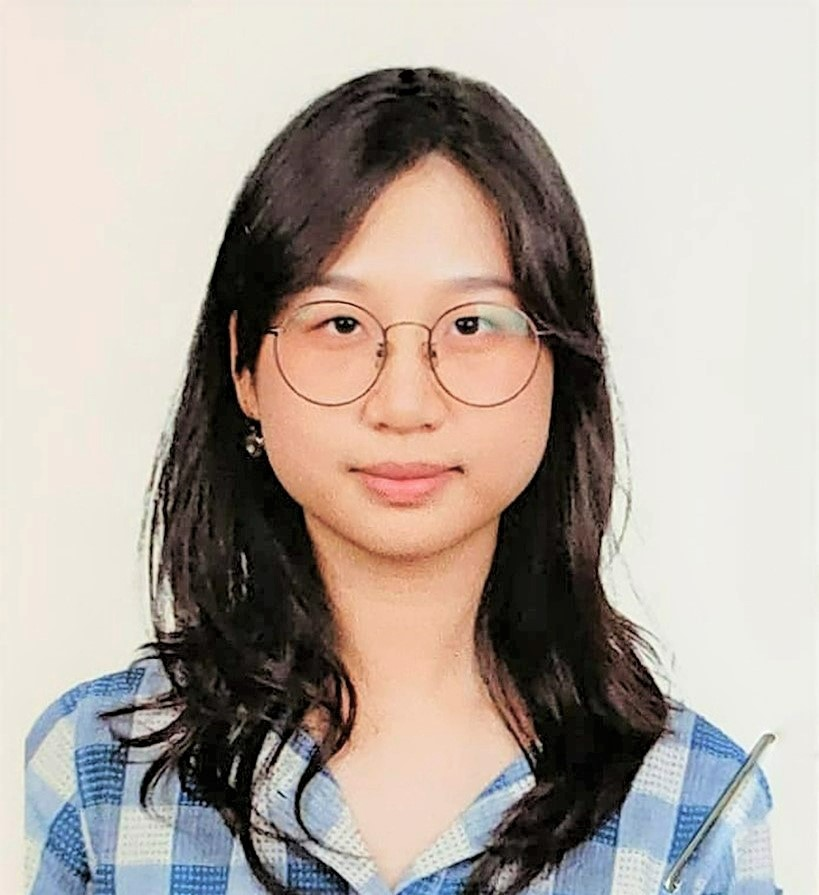
\includegraphics[width=2.0cm]{../profile-pic.jpg}
    \end{minipage}}  & {\textbf{\Large LIANA LING LI YA}} & \\
  & {\textit{Masters of Science (MSc) in Computer Science}} & {Email: \textbf{\href{mailto:lianalingliya@gmail.com}{lianalingliya@gmail.com}}} \\
  & {Apr 10, Phoenix Park Racecourse}, & {Mobile: \textbf{\href{tel:+60172801215}{+353 87 248 1446}}} \\
  & {Castleknock, D15 X381, Dublin 15} & {GitHub: \textbf{\href{http://github.com/lianaling/}{github.com/lianaling}}}\\
  & {Dublin, Ireland.} & {This Document: \textbf{\href{https://github.com/lianaling/resume/}{Coded with \LaTeX}}} \\
\end{tabular*}

%-----------Education-----------------
\section{EDUCATION}
\resumeSubHeadingListStart
\resumeSubheading
{University College Dublin}{Dublin, Ireland}
{Masters of Science (MSc) in Computer Science (Data Science); CGPA:3.78}{Sep 2023 -- Sep 2024}
% \begin{spacing}{0.4}
%   \colorbox{yellow}{\it\footnotesize CGPA: 3.9744}
% \end{spacing}
\resumeSubheading
{Tunku Abdul Rahman University of Management and Technology}{Kuala Lumpur, Malaysia}
{Bachelor of Computer Science (Honours) in Software Engineering; CGPA:3.98}{Oct 2019 -- Oct 2022}
% \begin{spacing}{0.4}
%   \colorbox{yellow}{\it\footnotesize CGPA: 3.9744}
% \end{spacing}
\resumeSubSubheading{Foundation in Science; CGPA: 4.00/4.00}{Sep 2018 -- Sep 2019}
\resumeSubHeadingListEnd

%-------------SKILLS-----------------
\section{SKILLS}
\resumeSubHeadingListStart
\resumeSubItem{\textbf{Programming: }}{Python, R, Julia, Microsoft Excel, Jupyter, Java, SQL}
\resumeSubItem{\textbf{Mathematics: }}{Data Analytics, Applied Statistical Modelling, Machine Learning, Data Management, Statistics and Probability, Monte Carlo Simulation, Quantitative Research Methods}
\resumeSubItem{\textbf{Languages: }}{Native-level English and Chinese; conversational in Malay and Cantonese}
\resumeSubHeadingListEnd

%-----------Experience-----------------
\section{EXPERIENCE}
\resumeSubHeadingListStart

\resumeSubheading
{Junior Quant Researcher}{Dec 2022 -- Sep 2023}
{Balaena Quant Sdn Bhd}{Kelana Jaya, Malaysia}
\resumeItemListStart
\resumeItem{}
{Worked with more than 1GB of \textbf{time-series} market data}
\resumeItem{}
{\textbf{Researched and designed} minute-level statistical arbitrage algorithms for crypto derivatives}
\resumeItem{}
{Wrote scripts to automate large-scale historical data insertion for crypto trading pairs}
\resumeItemListEnd

\resumeSubheading
{Machine Learning Intern}{June 2022 -- Nov 2022}
{Datasonic Smart Solutions Sdn Bhd}{Putrajaya, Malaysia}
\resumeItemListStart
\resumeItem{}
{Studied journal papers on \textbf{speech recognition and computer vision}}
\resumeItem{}
{\textbf{Managed data from collection, manipulation and augmentation} for training ML models}
\resumeItem{}
{Trained CNN's variant (YOLOv7) to perform card detection using PyTorch}
\resumeItem{}
{Designed UI for an OAuth system and connected to backend using VueJS and Quasar}
\resumeItemListEnd
\resumeSubHeadingListEnd


%-----------Projects-----------------
\section{PROJECTS}
\resumeSubHeadingListStart

\resumeSubheading{Prediction of Advanced Prostate Cancer}{Statistical Analysis}
{R Language}{Mar 2024 -- Apr 2024}
\resumeItemListStart
\resumeItem{}
{Performed data analysis on real-life patient data: \textbf{boxplots, correlation, interaction plots}, etc.}
\resumeItem{}
{Identified and dealt with \textbf{non-linearity} via \textbf{Box-Tidwell test}}
\resumeItem{}
{Applied logistic regression to \textbf{model the impact of factors} on the probability of being diagnosed with advanced prostate cancer}
\resumeItemListEnd

\resumeSubheading{Air Pollution Analysis in the US}{Statistical Analysis}
{R Language}{Feb 2024 -- Mar 2024}
\resumeItemListStart
\resumeItem{}
{Identified \textbf{multicollinearity} via flipping of signs in regression coefficients}
\resumeItemListEnd

\resumeSubheading{Cost Analysis of Nuclear Plant Construction in the US}{Statistical Analysis}
{R Language}{Feb 2024 -- Mar 2024}
\resumeItemListStart
\resumeItem{}
{\textbf{Assessed model validity} by analysing model residuals}
\resumeItem{}
{Improved model fit to \textbf{an $R^2$ of 0.92 and adj. $R^2$ of 0.85} by including interaction terms}
\resumeItem{}
{Identified important factors that increased the cost of nuclear plant construction}
\resumeItemListEnd

\resumeSubheading{\href{https://github.com/lianaling/connectionist-computing}{Feedforward Neural Network From Scratch}}{Machine Learning}
{Python}{Nov 2023 -- Dec 2023}
\resumeItemListStart
\resumeItem{}
{Implemented an extendable library for customisable neural network architecture}
\resumeItem{}
{Obtained 80\% test accuracy on the \href{https://archive.ics.uci.edu/dataset/59/letter+recognition}{UCI letter recognition dataset}}
\resumeItemListEnd
\resumeSubHeadingListEnd


%-----------Academia-----------------
\section{ACADEMIA}
 {\small
  \begin{itemize}[leftmargin=*]{\footnotesize}
    \item{Ling, L., Amirul Imran Ahmad Azam, Ramanathan Palaniappan, \& Tin, T.T. (2021, November 25-27) \textit{Artificial Intelligence Art: Attitudes and Perceptions Toward Human Versus Artificial Intelligence Artworks.} [Paper presentation]. ICHESMET 2021. \vspace{-2pt}}
  \end{itemize}
 }


%-----------Achievements-----------------
\section{ACHIEVEMENTS}
\resumeSubHeadingListStart
\resumeSubItem{UCD Global Excellence Scholarship }{(top academic performance)}
\resumeSubItem{TAR UMT President's Award }{(valedictorian/top performing student)}
\resumeSubItem{TAR UMT President's List certificates }{(GPA 3.9000 and above)}
\resumeSubItem{TAR UMT Full Academic Scholarship }{(foundation and bachelor's degree)}
\resumeSubItem{Band 8.5 on a -band scale for IELTS 2022}{}
\resumeSubHeadingListEnd


%-------------------------------------------
\end{document}

% -----Credits-----
% Template: Sourabh Bajaj
% License : MIT